\documentclass[12pt,a4paper]{report}
 
\usepackage[hmargin=1in,vmargin=1in]{geometry}
\usepackage{amsmath}
\usepackage{graphicx}
\usepackage{fancyhdr}


 \newcommand{\stud}{Kurian C Kurian} 
 \newcommand{\roll}{Roll numbe} 
 \newcommand{\dept}{\large\textbf{Department of Electronics \& Communication}} 
 \newcommand{\instis}{ER \& DCIInstitute of Technology, Vellayambalam, Thiruvananthapuram} 
 \newcommand{\depts}{\textbf{Department of Electronics \& Communication}} 
 \newcommand{\stream}{\emph{VLSI $\&$ EMBEDDED SYSTEMS}} 
 \newcommand{\degree}{Master of Technology} 
 \newcommand{\uni}{APJ Abdul Kalam Technological University} 
 \newcommand{\projectname}{``Attention Tracker "} 
 \newcommand{\projectnameb}{Attention Tracker} 
 \newcommand{\insti}{ER\&DCI Institute of Technology
\\ Centre for Development of Advanced Computing (CDAC)
\\ Vellayambalam, Thiruvananthapuram.
\\ Kerala, India - 695033} 
\newcommand{\salu}{Mr.} 
\newcommand{\guide}{\salu{} Kadar A. A.} 

\renewcommand{\baselinestretch}{1.5}
\setlength{\parindent}{1em}
\setlength{\parskip}{1em}

\begin{document}


\thispagestyle{empty}
\begin{center}
{\Large{\textbf{\projectnameb{}}}}
\vspace{5mm}
\\ \MakeUppercase{\reportTitle{} report}
\vspace{5mm}
\\submitted by
\\\stud{}
\vspace{5mm}
\\ \dept{} 
\\{\textbf{Reg No:\roll{}}}
\vspace{5mm}
\\to
\\the APJ Abdul Kalam Technological University
\\in partial fulfillment of the requirements for the award of the Degree
\\of
\\ \degree{}
\\in
\\ \stream{}
\end{center}

\begin{figure}[ht]
\centering

\includegraphics[scale=0.5]{logo}
\end{figure}

\begin{center}
{\dept{}
\vspace{5mm}
\insti{}}
\end{center}

\newpage
\thispagestyle{empty}

\begin{center}
\textbf{DECLARATION}
\end{center}


I undersigned hereby declare that the seminar report ``\projectname{}" 
, submitted for the partial fulfillment of the requirements for the award of degree of \degree{} of the APJ Abdul Kalam Technological University, Kerala is a bonafide work done by me under the supervision of \guide{}. This submission represents my ideas in my own words and where ideas or words of others have been included, I have adequately and accurately cited and referenced the original sources. I also declare that I have adhered to ethics of academic honesty and integrity and have not misrepresented or fabricated any data or idea or fact or source in my submission. I understand that any violation of the above will be a cause for disciplinary action by the institute and/or the University and can also evoke penal action from the sources which have thus not been properly cited or from whom proper permission has not been obtained. This report has not been previously formed the basis for the award of any degree, diploma or similar title of any other University. 
\vspace{20mm}
\\Place: Trivandrum								
\\Date: dd-mm-yyyy     \hfill     \stud{} 

\newpage
\thispagestyle{empty}
\begin{center}
{\insti{}}

\begin{figure}[ht]
\centering

\includegraphics[scale=0.5]{logo}
\end{figure}
{\large{\textbf{CERTIFICATE}}}

\end{center}

This is to certify that the report entitled,\textbf{ \projectname{}} submitted by \textbf{\stud{}} to the \uni{} in the partial fulfillment of the requirements for the award of the Degree of \degree{} in \stream{}, \depts{} is a bonafide record of the project work carried out by her under our guidance and supervision. This report in any form has not been submitted to any other University or Institute for any purpose.
\vspace{25mm}
 \\         
\begin{flushright} Project Guide \end{flushright} 
                                                                                     

\newpage
\pagenumbering{roman}
\begin{center}
\textbf{ACKNOWLEDGEMENT}
\end{center} 
My endeavour stands incomplete without dedicating my gratitude to everyone who has
contributed lot towards the successful completion of my seminar report. I am in debited
to my parents for blessing me with their grace and taking my endeavor to a successful
culmination. I express my gratitude to \textbf{\guide{}}, \textbf{principal \prince{}}, \instis{} for all the help rendered
to me. I also thank all the faculties of my college for the help they have extended. I
extend my sincere thanks to \textbf{\guide{}},\reportTitle{} guide for providing me with the guidance and facilities for the \reportTitle{} . I
express my sincere gratitude to seminar coordinator \textbf{\coord{}}, for his cooperation and guidance for preparing and presenting this \reportTitle{}
report.
 

\newpage
\begin{center}
\textbf{ABSTRACT}
\end{center}  

	This project is an implementation of Opencv in real world. It uses, Raspberrypi for easy replication and portability. The module, works
by capturing images of objects, temporarily storing them on disk and processing them to see if image of a face exists in
the stored image. After detection stored images is immediately deleted or over written to conserve space. 

From opencv we use feature extraction a feature extraction method, which subtracts pixels of a group(identified by the algorithm) from
the original image, to form a pattern object. This pattern object is then subjected to neural network to check if it fits the pattern of a face.



\tableofcontents
\listoffigures
\newpage

%\pagestyle{fancy}

%\rhead{Share\LaTeX}
%\lhead{Guides and tutorials}
\section{Introduction}
Attention Tracker is a module which can be installed independently on show cases, merchandise, posters to see which product is getting maximum attention from people. It is completely unobtrusive unlike survey forms and feebdack requests and therefore can be more effective. It uses Face recognition software called opencv, an image processing algorithm, and neural network. This application is on top of
raspbian os which controls the frequency of monitoring, raspbian os is an open source oeprating system for raspberrypi, based on linux kernel. It is a branch of debian OS. The module, works by capturing images of objects, temporarily storing them on disk and processing them to see if image of a face exists in the stored image. After detection stored images is immediately deleted or over written to conserve space. 

From opencv we use feature extraction a feature extraction method, which subtracts pixels of a group(identified by the algorithm) from
the original image, to form a pattern object. This pattern object is then subjected to neural network to check if it fits the pattern of a face. It is based on the work done by Witsarut Sriratana et al\cite{8434429}.

\section{Litratrue Survey}
In the paper \cite{opencv} W.Sriratana et al. presents a face identification system. It works by capturing image in real time, converting that image to integral image,
and running Feature extraction Function on it. The Feature extraction function searches for standard facial features like dark regions around eyes, light regions at the nose. The output of this function
is a set of patterns, which may or may not predict if given image has a face. This output is then input to a neural network, which is trained to identify if there is a face. Each feature vector is given its weight according to its aility to predict a feature

viola jones algorithm \cite{violajones} is aimed at speeding up face recognition. Face recognition, involves finding difference in
pixel intensities between rectangular blocks of pixels. what viola jones algorithm does is to create an intermediate image called
the integral image which is easier to operate on. The integral image significantly speeds up face recognition techniques. It does
this by reducing the number of times a value is accessed from the disk to calculate an image feature.


\begin{figure}[ht]
\centering
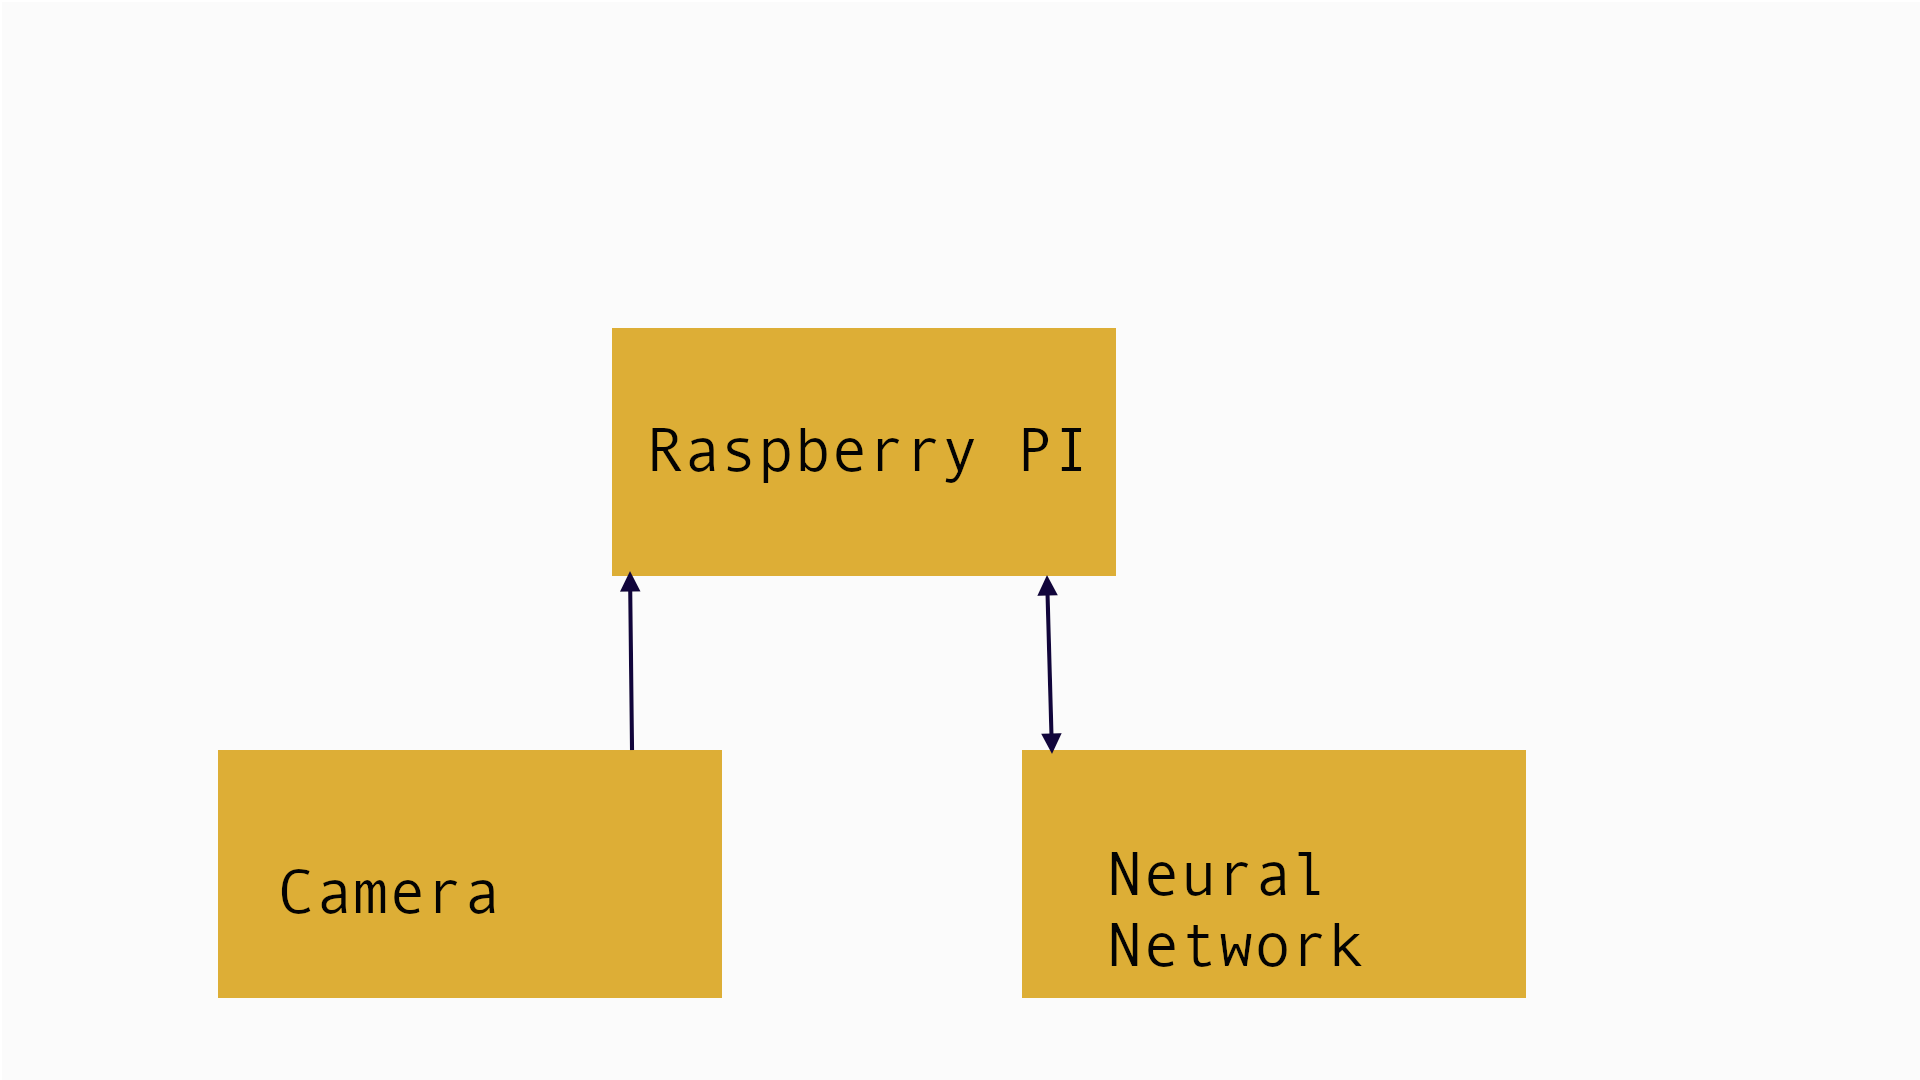
\includegraphics[scale=0.7]{block}
\caption{Different components of attention tracker}
\end{figure}

\section{Raspberry PI}
The Raspberry PI is a small single-board computer. It is developed by Raspberry PI Foundation to promote teaching of basic computer science in schools. It has  1.2 GHz 64-bit quad core processor, on-board 802.11n Wi-Fi, Bluetooth and USB boot capabilities. 

\section{Image Processing}
Neural network includes Image preprocessing block, feature extraction block and an implementation of deep learning network. Image processing works by convering the given image to integral image.

\subsection{Neural Network}
Neural network is a series of weigted functions. These functions give output based on the threshold function. The threshold function can be softmax or spiking neural network etc.  This can be used to detect features
of image which can determine whether a given image has a face or not. This is done by
training neural network on known images, which have faces and adjusting weights to reduce false positives. In put to neural network is an integral image. Which is better
at detecting face than traditional methods like primary component vector analysis, which operate on entire image.
\subsection{Integral Image}
Integral image is the concept introduced by Viola Jones et al. It makes image processing faster. It is done by subjecting all the pixels of image to the following set of transformations.
\begin{align*}
    IntegralImage(x,y) &=Image(x,y)+IntegralImage(x-1,y)+IntegralImage(x,y-1)\\
    IntegralImage(x,-1) &=0\\
    IntegralImage(-1,0) &=0\
\end{align*}
The resulting $IntegralImage$ makes it faster to perform image detection functions like the Haar Function. The Haar function selects rectangular regions in an image, and finds their difference from other rectangular region.
\begin{figure}[ht]
\centering
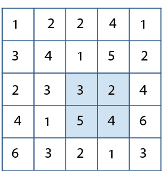
\includegraphics[scale=0.7]{image}
\caption{image with pixels represented by numbers}
\end{figure}

\begin{figure}[ht]
\centering
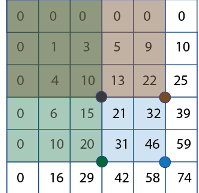
\includegraphics[scale=0.7]{iimage}
\caption{integral image}
\end{figure}



\newpage
\section{Schematic}

Raspberry Pi (/paɪ/) is a single-board computer developed in the United Kingdom by the Raspberry Pi Foundation to promote teaching of basic computer science in schools and in developing countries.The original model clocked at 700Mhz, had composite video output and no wifi, it became popular selling outside its target market for uses such as robotics. 

The first generation (Raspberry Pi 1 Model B) was released in February 2012, followed by the simpler and cheaper Model A. In 2014, the Foundation released a board with an improved design, Raspberry Pi 1 Model B+. These boards are approximately credit-card sized and represent the standard mainline form-factor. Improved A+ and B+ models were released a year later. A "Compute Module" was released in April 2014 for embedded applications. The Raspberry Pi 2, which added more RAM, was released in February 2015.

Raspberry Pi 3 Model B was released in February 2016 with a 1.2 GHz 64-bit quad core processor, on-board 802.11n Wi-Fi, Bluetooth and USB boot capabilities.It has gigabit Ethernet (throughput limited to ca. 300 Mbit/s by the internal USB 2.0 connection) or 2.4 / 5 GHz dual-band 802.11ac Wi-Fi (100 Mbit/s). Other features are Power over Ethernet (PoE) (with the add-on PoE HAT), USB boot and network boot (an SD card is no longer required).
\begin{figure}[ht]
\centering
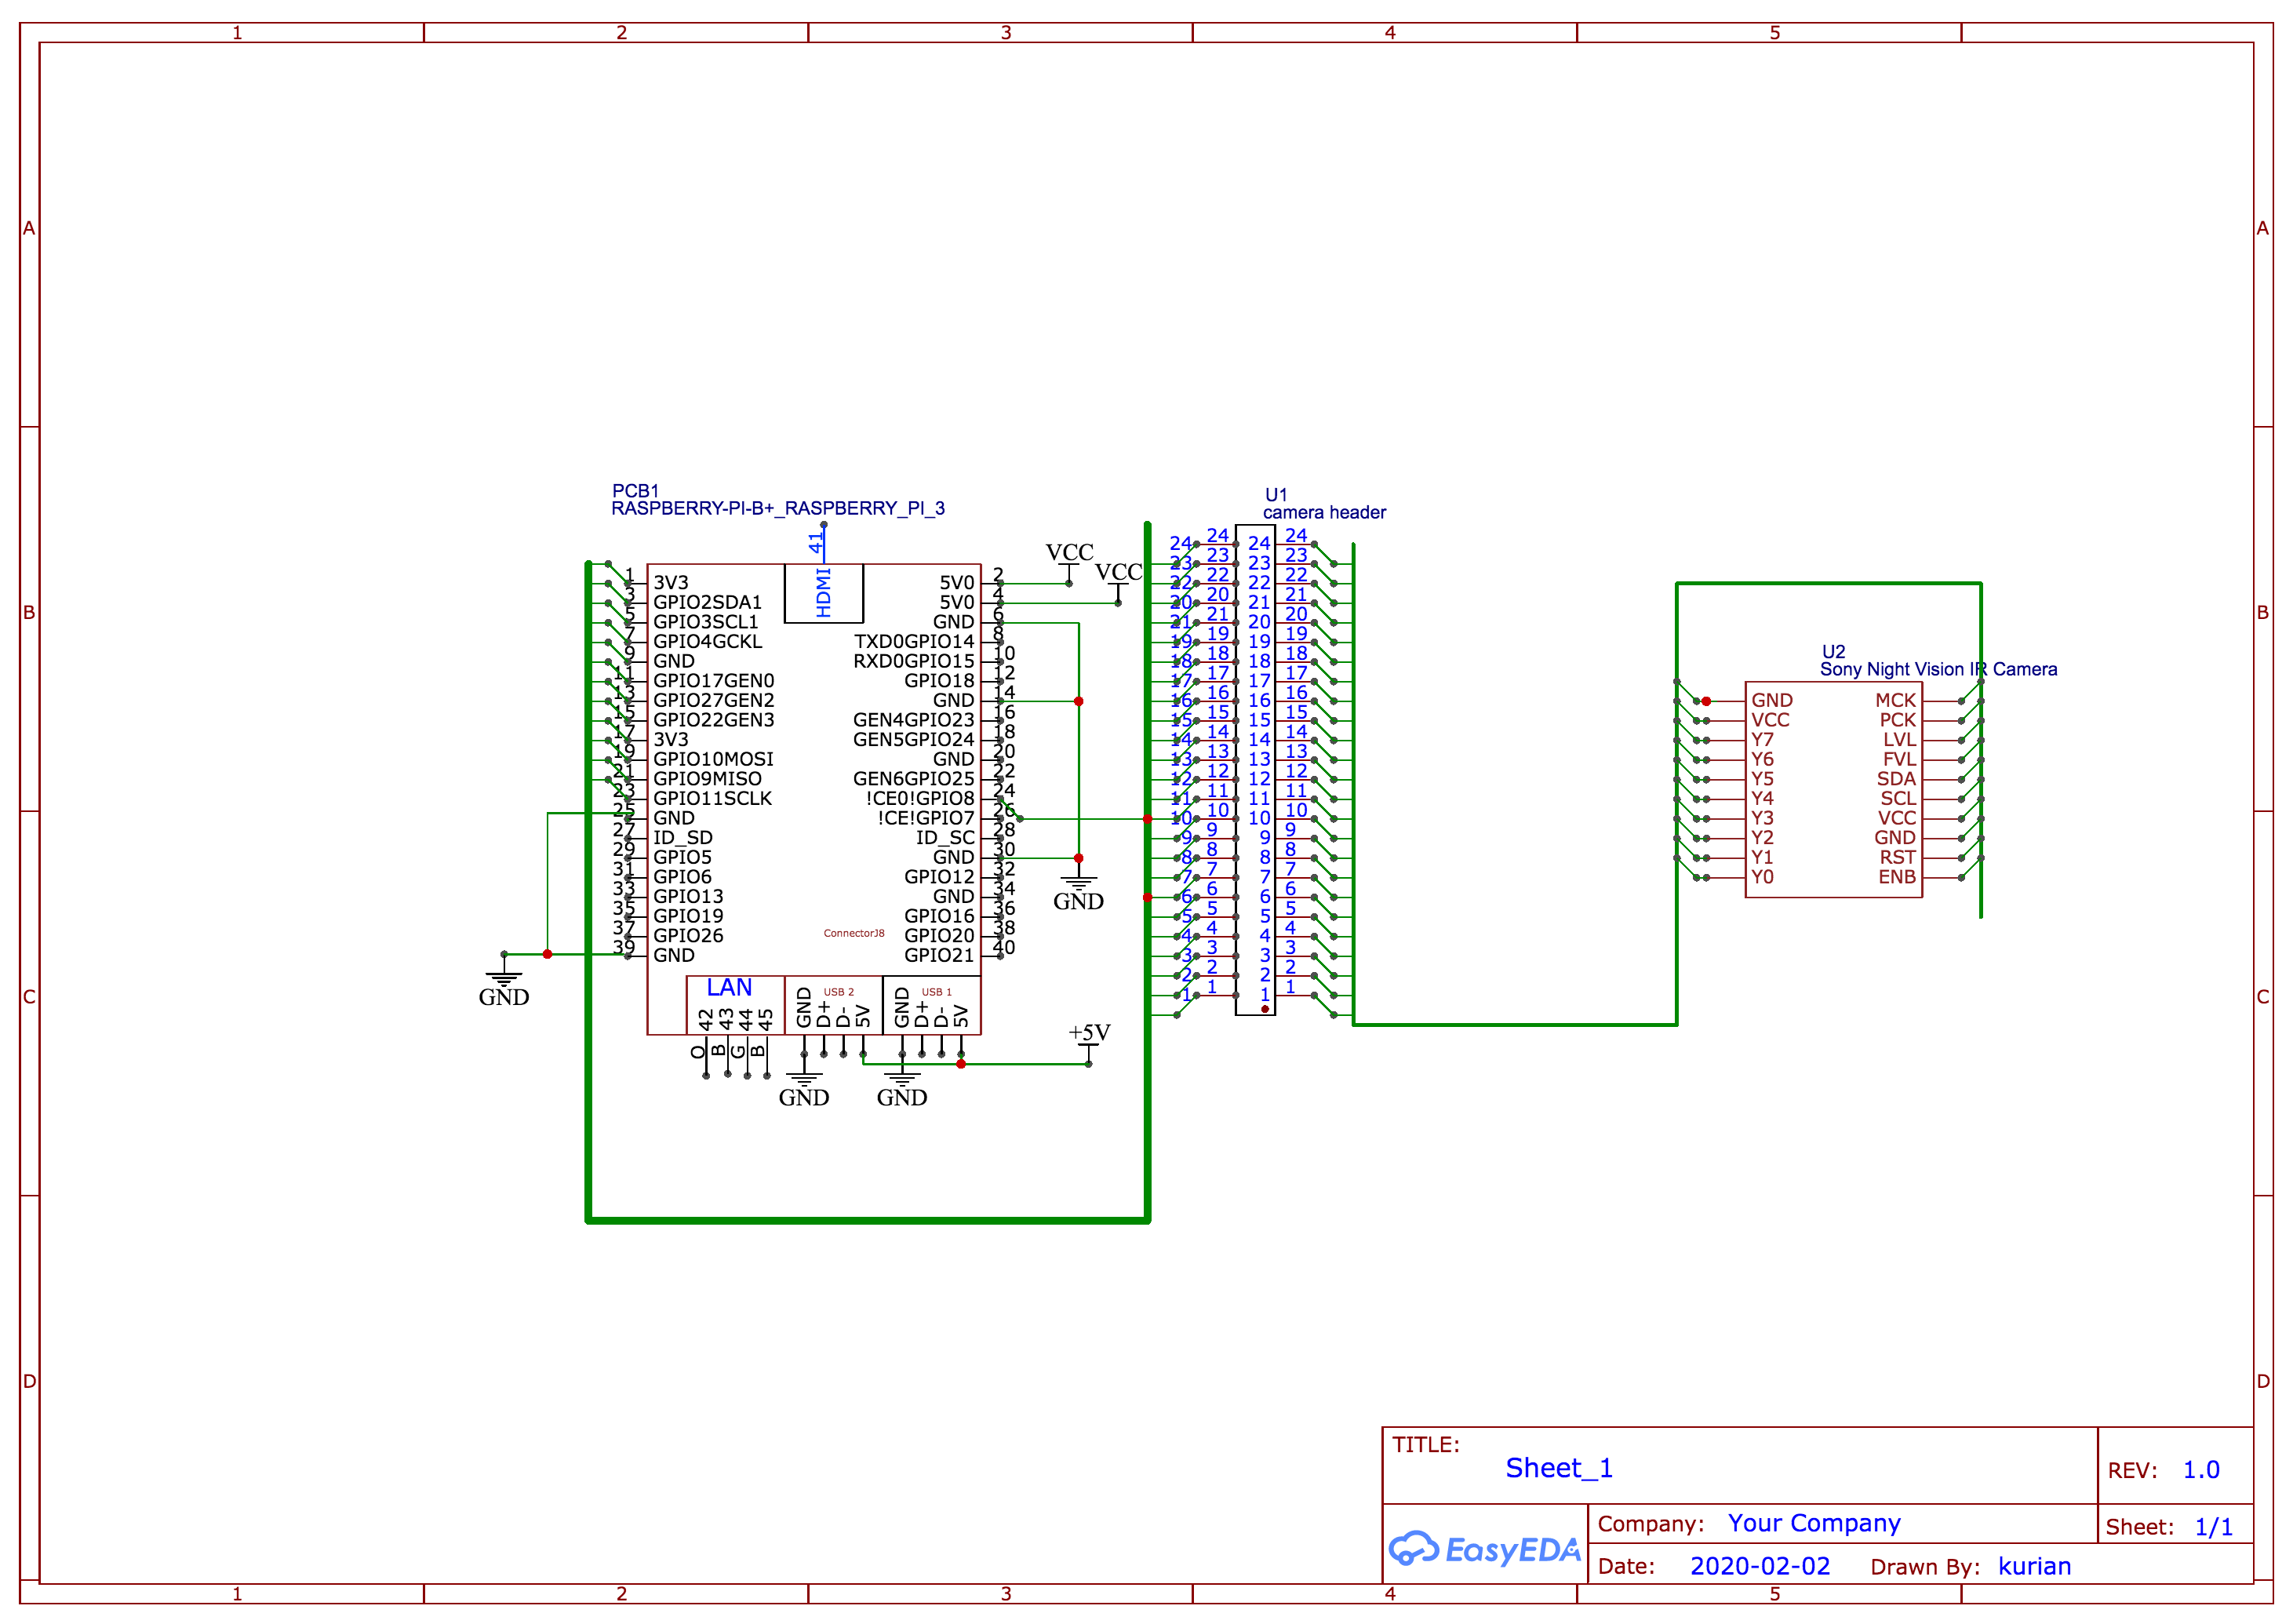
\includegraphics[scale=0.15]{project}
\caption{Schematic of attention tracker}
\end{figure}

\newpage
In order to build attention tracker, a Raspberry PI board was obtained, Raspbian Os was installed. In order to implement attention tracker, Viola Jones algorithm was selected. Open CV functionality was tested on host machine to implement image capturing functionality. The system proposed in this project is not available today. 


\bibliography{ref} 
\bibliographystyle{ieeetr}
\end{document}
